\documentclass{beamer}

\usepackage[english]{babel}
\usepackage[utf8x]{inputenc}
\usepackage{amsmath,amsfonts,amssymb}

\usepackage{mathtools}


\usepackage{subcaption}

\usepackage[absolute,overlay]{textpos}





\newcommand{\todo}[1]{\textcolor{red}{TODO: #1}}

\addtobeamertemplate{navigation symbols}{}{%
    \usebeamerfont{footline}%
    \usebeamercolor[fg]{footline}%
    \hspace{1em}%
    \insertframenumber/\inserttotalframenumber
}

\setbeamertemplate{bibliography item}[text]
\bibliographystyle{unsrt}


\usetheme{Luebeck}
\usecolortheme{orchid}

\title[Current state of master thesis]{Parameter estimation of specific heat capacity $c_p$ at phase change using a model \\ of a heat flux DSC.}
\subtitle{Current state of master thesis}

\author{Jan Lammel}

\begin{document}
	
\frame{\titlepage}

\frame{
	\frametitle{Table of contents}
	\tableofcontents[hideallsubsections]
	
}

\section{Introduction}
\frame{
\frametitle{Introduction}

	\begin{textblock}{7}(1,5)
		\includegraphics[width=1.0\textwidth]{/home/argo/masterarbeit/thesis/images/handwaermer[wiki].jpg} \\
		\qquad \quad Source: Wikipedia
	\end{textblock}
	
	\begin{textblock}{8}(8,5)
	\begin{itemize}
		\item We examine so called phase change materials (PCM)
		\item Important property is the heat capacity $c_p$: When does it melt and how much energy fits into?
	\end{itemize}
	\end{textblock}

	\begin{textblock}{14}(1,12.5)

	\textbf{Goal:} Simulation of measuring process to obtain specific heat capacity $c_p$ of phase change material (PCM) by parameter estimation.

	\end{textblock}
	

}

\section{Physics}
\subsection{Important physical quantities}
\frame{
	\frametitle{Important physical quantities}
	
	\begin{textblock}{14}(1,5)
		\begin{itemize}
			\item Heat $Q$, \qquad $[Q] = J$ \\
			Amount of energy transferred because of temperature difference \\ \vspace{0.2cm}
			\item heat flux density $\Phi_q$, \qquad$[\Phi_q] = \frac{W}{m^2}$ \\
			Rate of energy transferred per unit area \vspace{0.2cm}
			\item specific heat capacity $c_p$, \qquad $[c_p] = \frac{J}{kg \cdot K}$ \\
			Material specific amount of energy needed to raise the temperature of $1kg$ by $1K$
			
		\end{itemize}
	\end{textblock}
	
}


\subsection{Heat flux differential scanning calorimetry (DSC)}
\frame{
	\frametitle{Heat flux differential scanning calorimetry (DSC)}
	
	\begin{textblock}{15}(0.4,4)
		\centering
		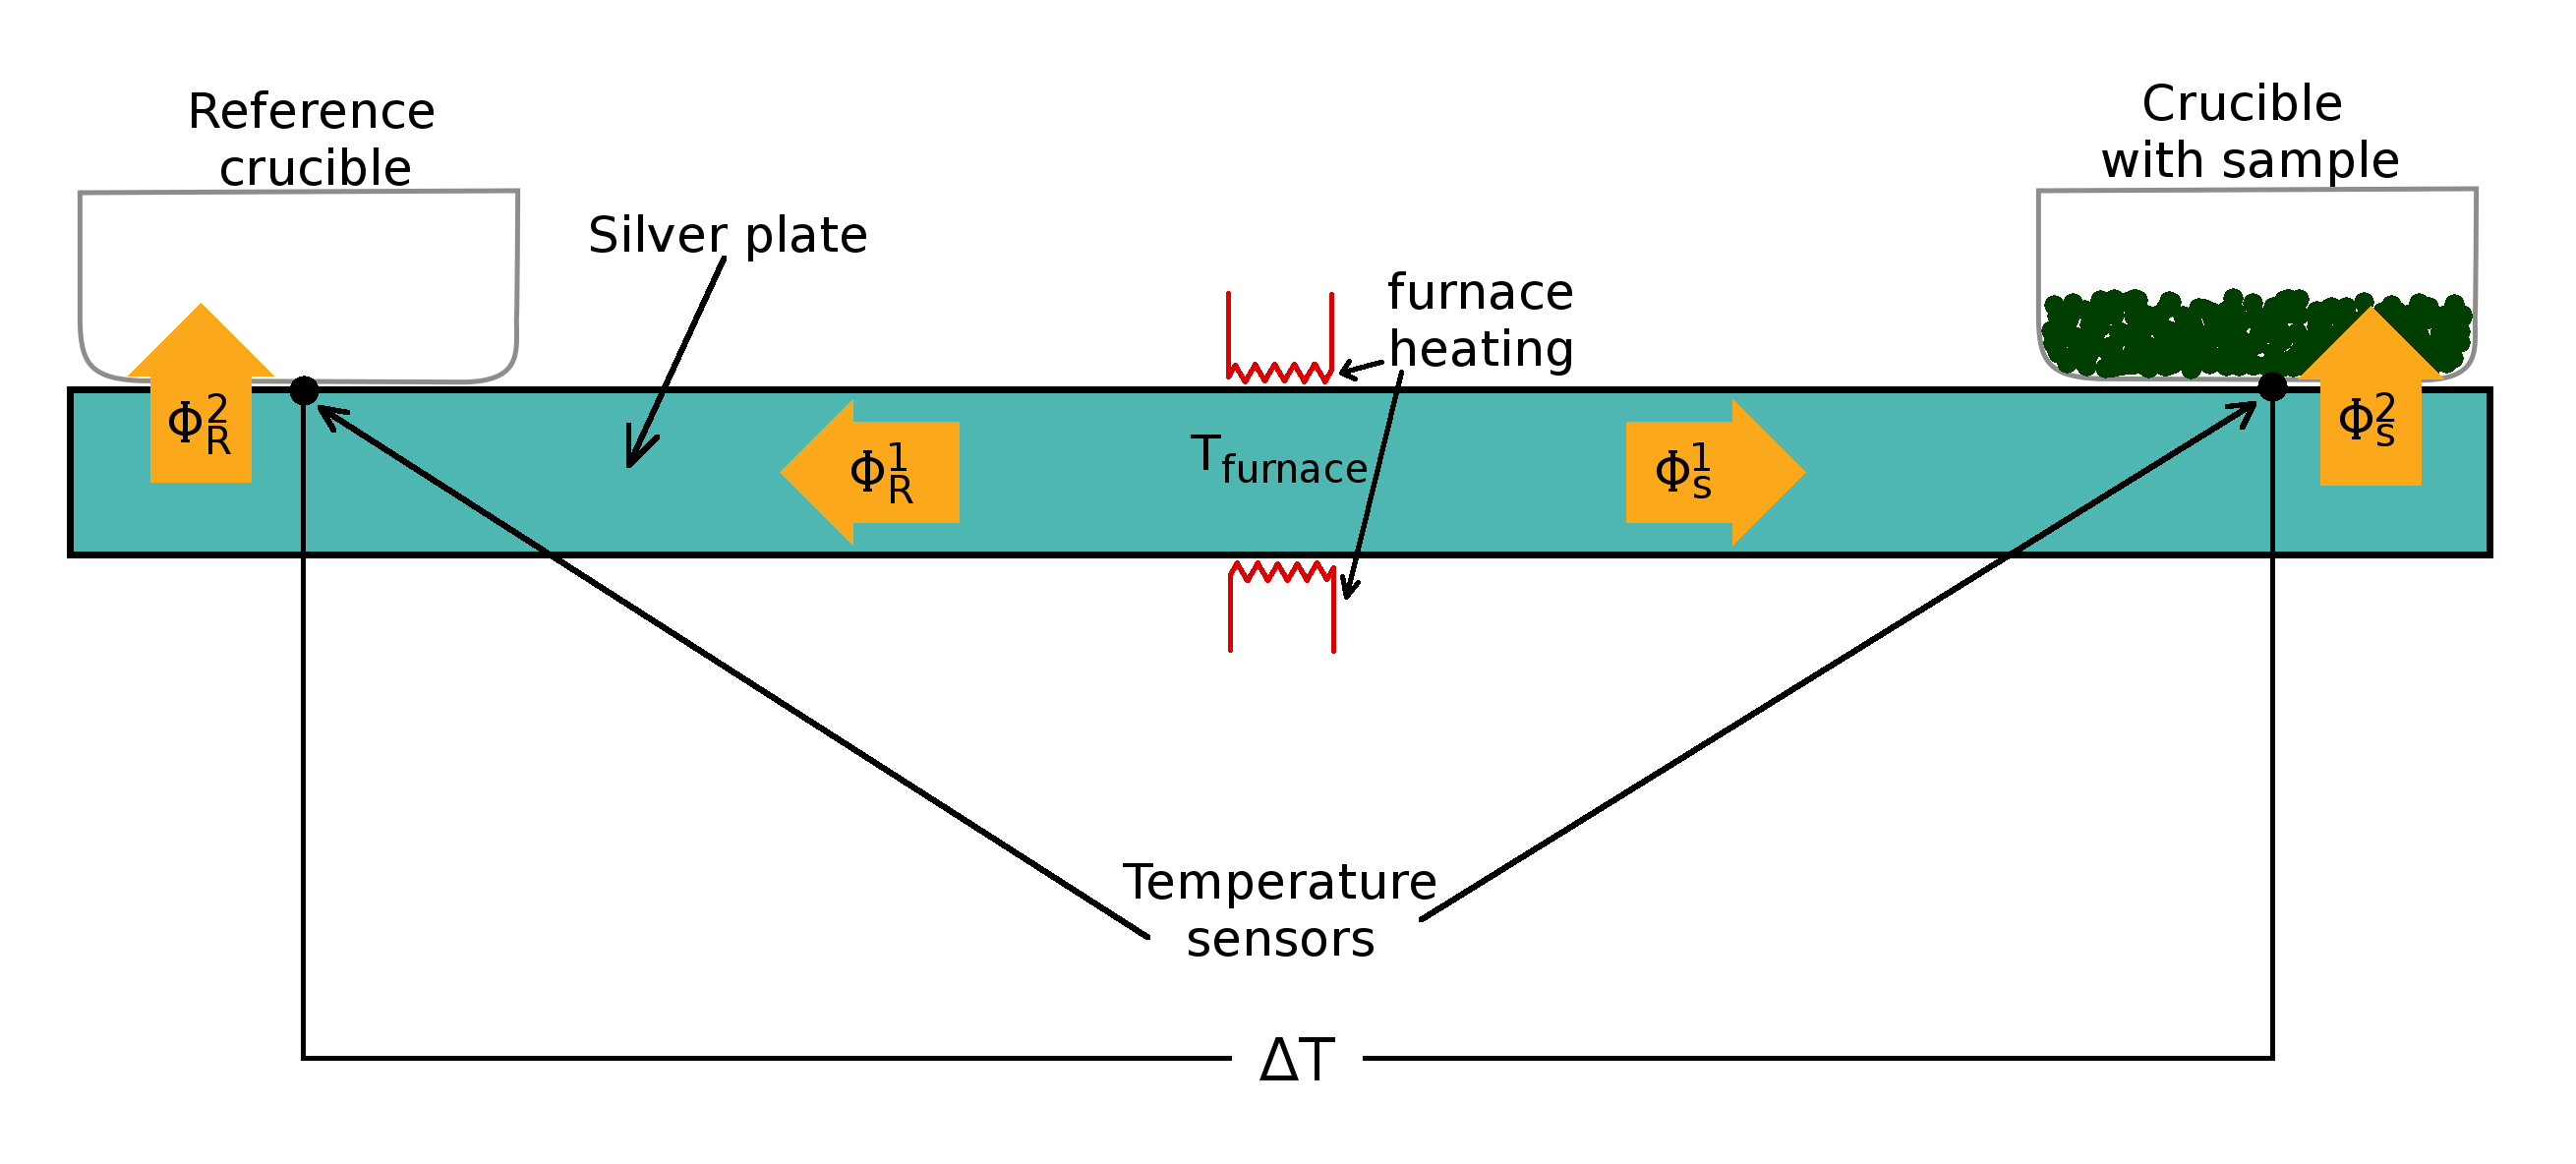
\includegraphics[width=0.7\textwidth]{/home/argo/masterarbeit/thesis/images/dsc_funktionsprinzip.png}
		
		\begin{itemize}
			\item Empty reference crucible and crucible with PCM are heated equally
			\item Due to thermal properties differences (mainly $c_p$) of reference and PCM a temperature difference $\Delta T$ is induced
			\item Sensitivity calibration with materials of known thermal properties provides mapping $\Delta T \rightarrow \Phi_q$
		\end{itemize}
		
	\end{textblock}
	
}


\subsection{Smearing problem}
\frame{
	\frametitle{Smearing problem}	
	
	\begin{textblock}{10}(0.5,5)
		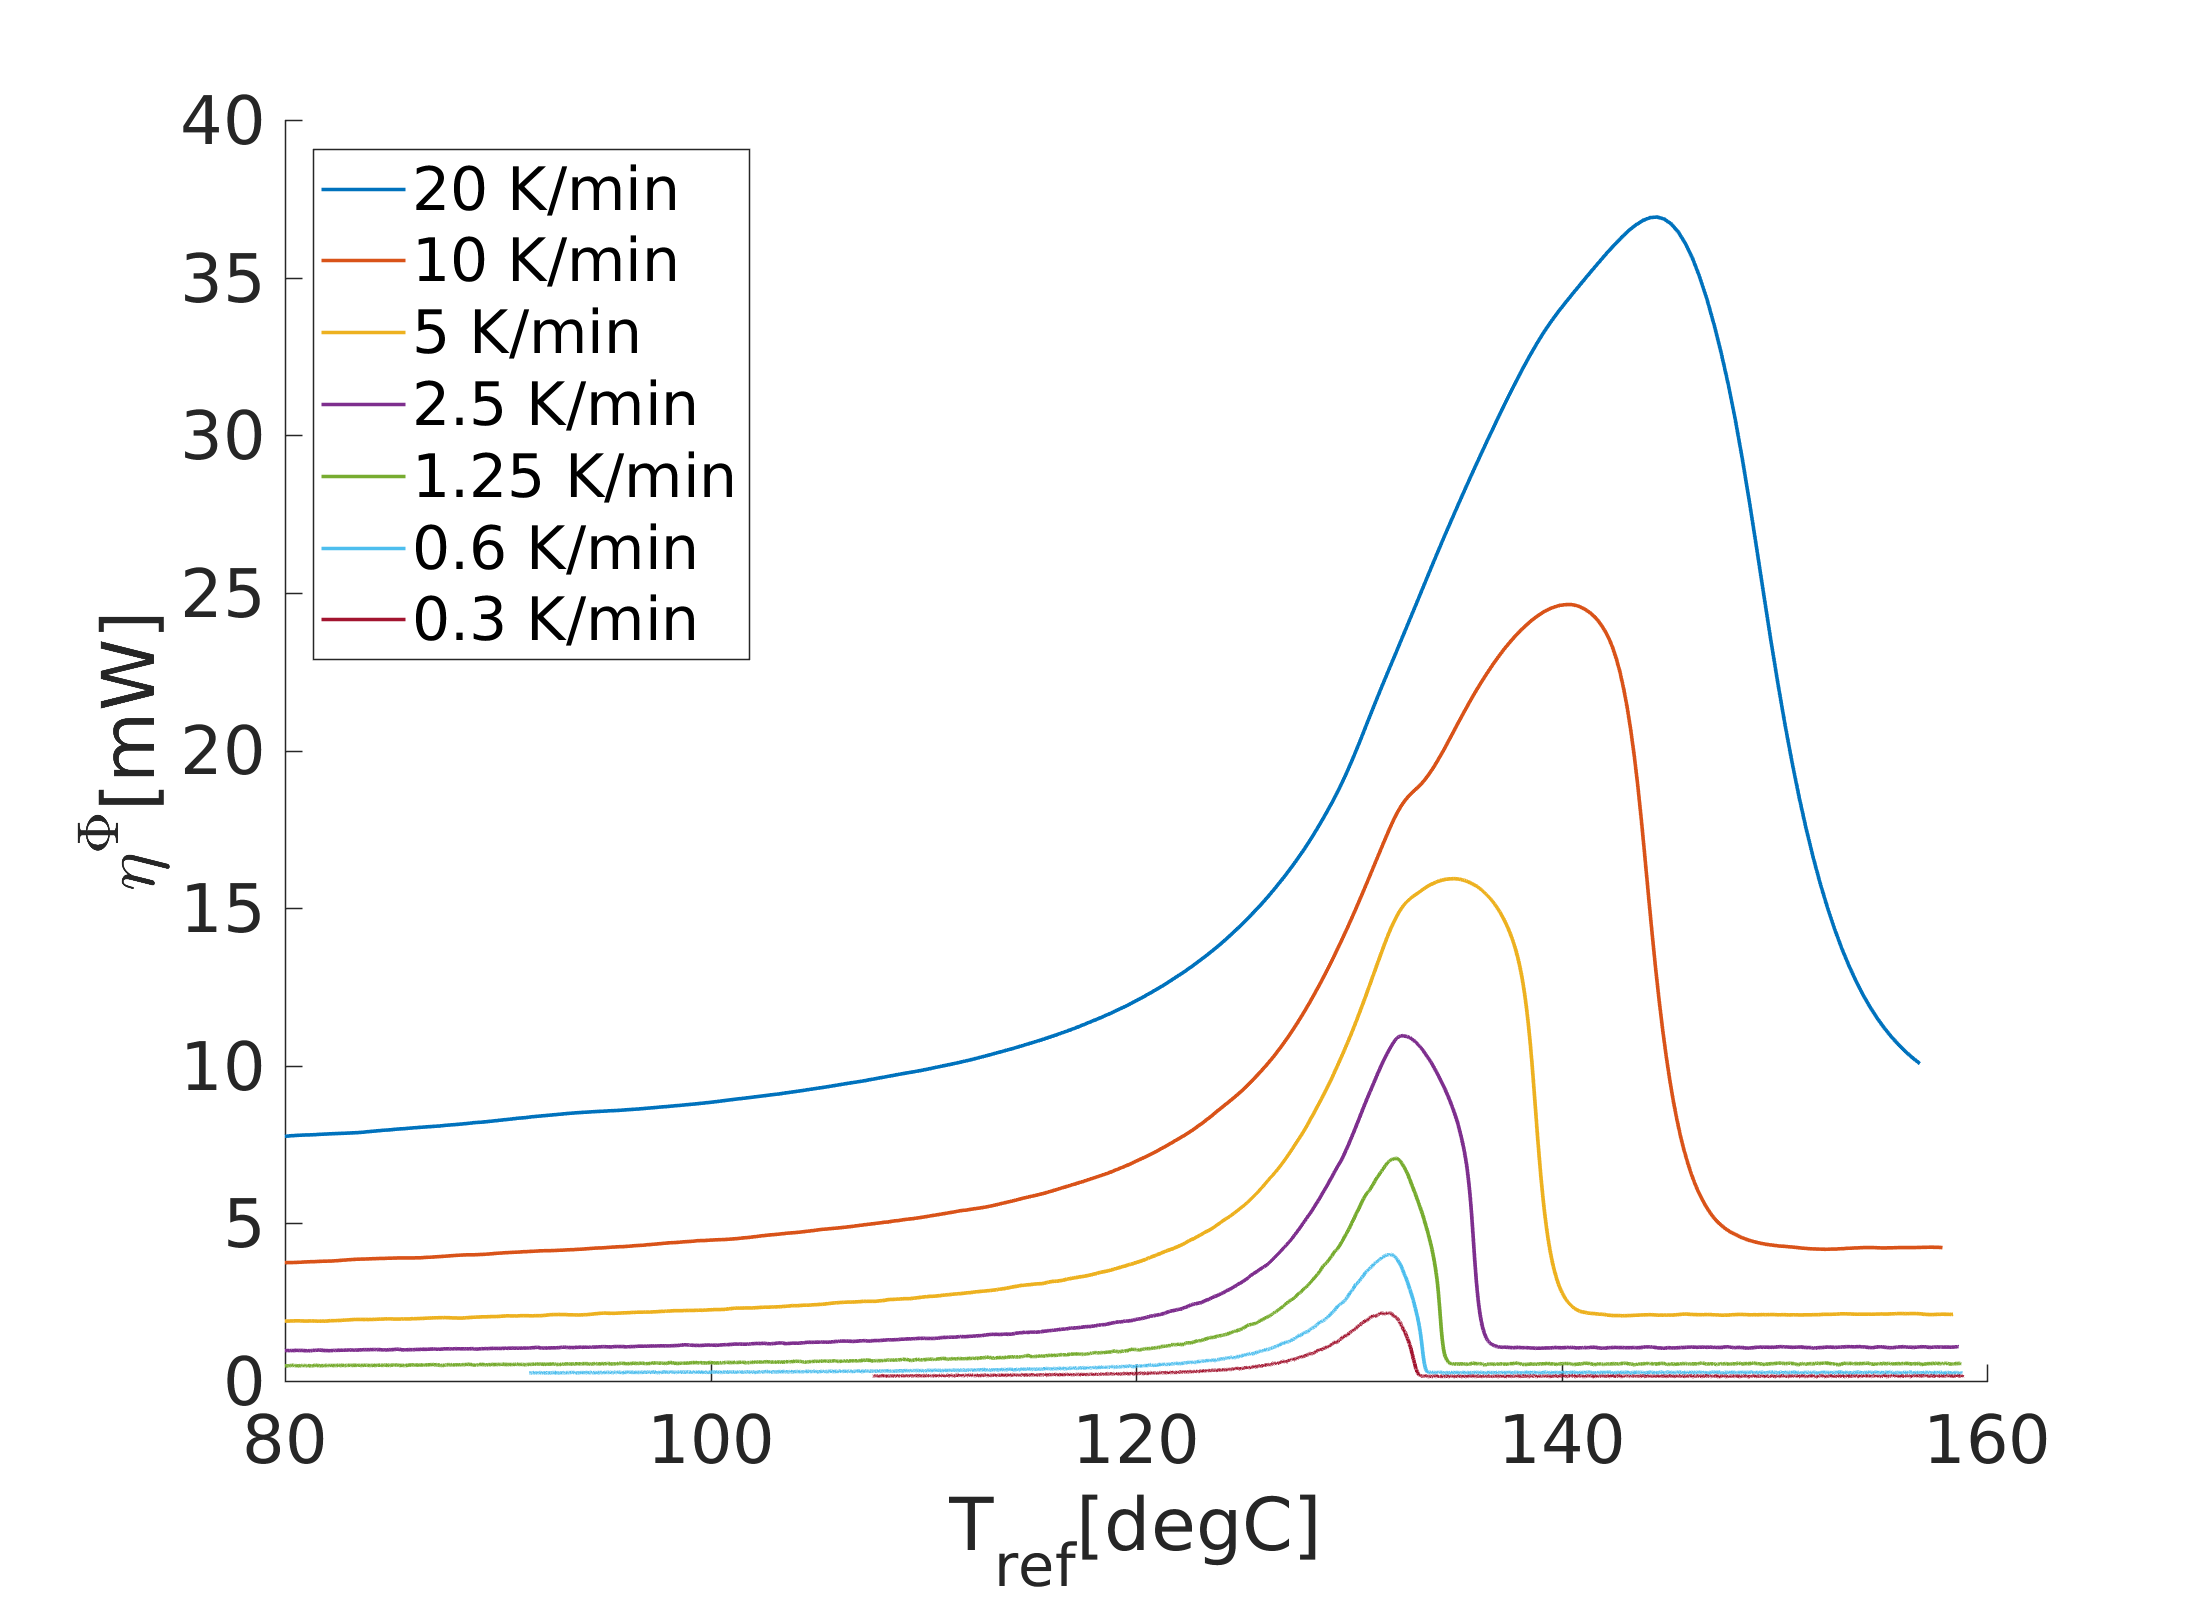
\includegraphics[width=0.7\textwidth]{/home/argo/masterarbeit/vortrag/images/heat_flux_measurement.png}
	\end{textblock}
	
	\begin{textblock}{4}(7.5,8)
		$\stackrel{(1)}{\longrightarrow}$
	\end{textblock}
	
	\begin{textblock}{10}(8.7,5)
		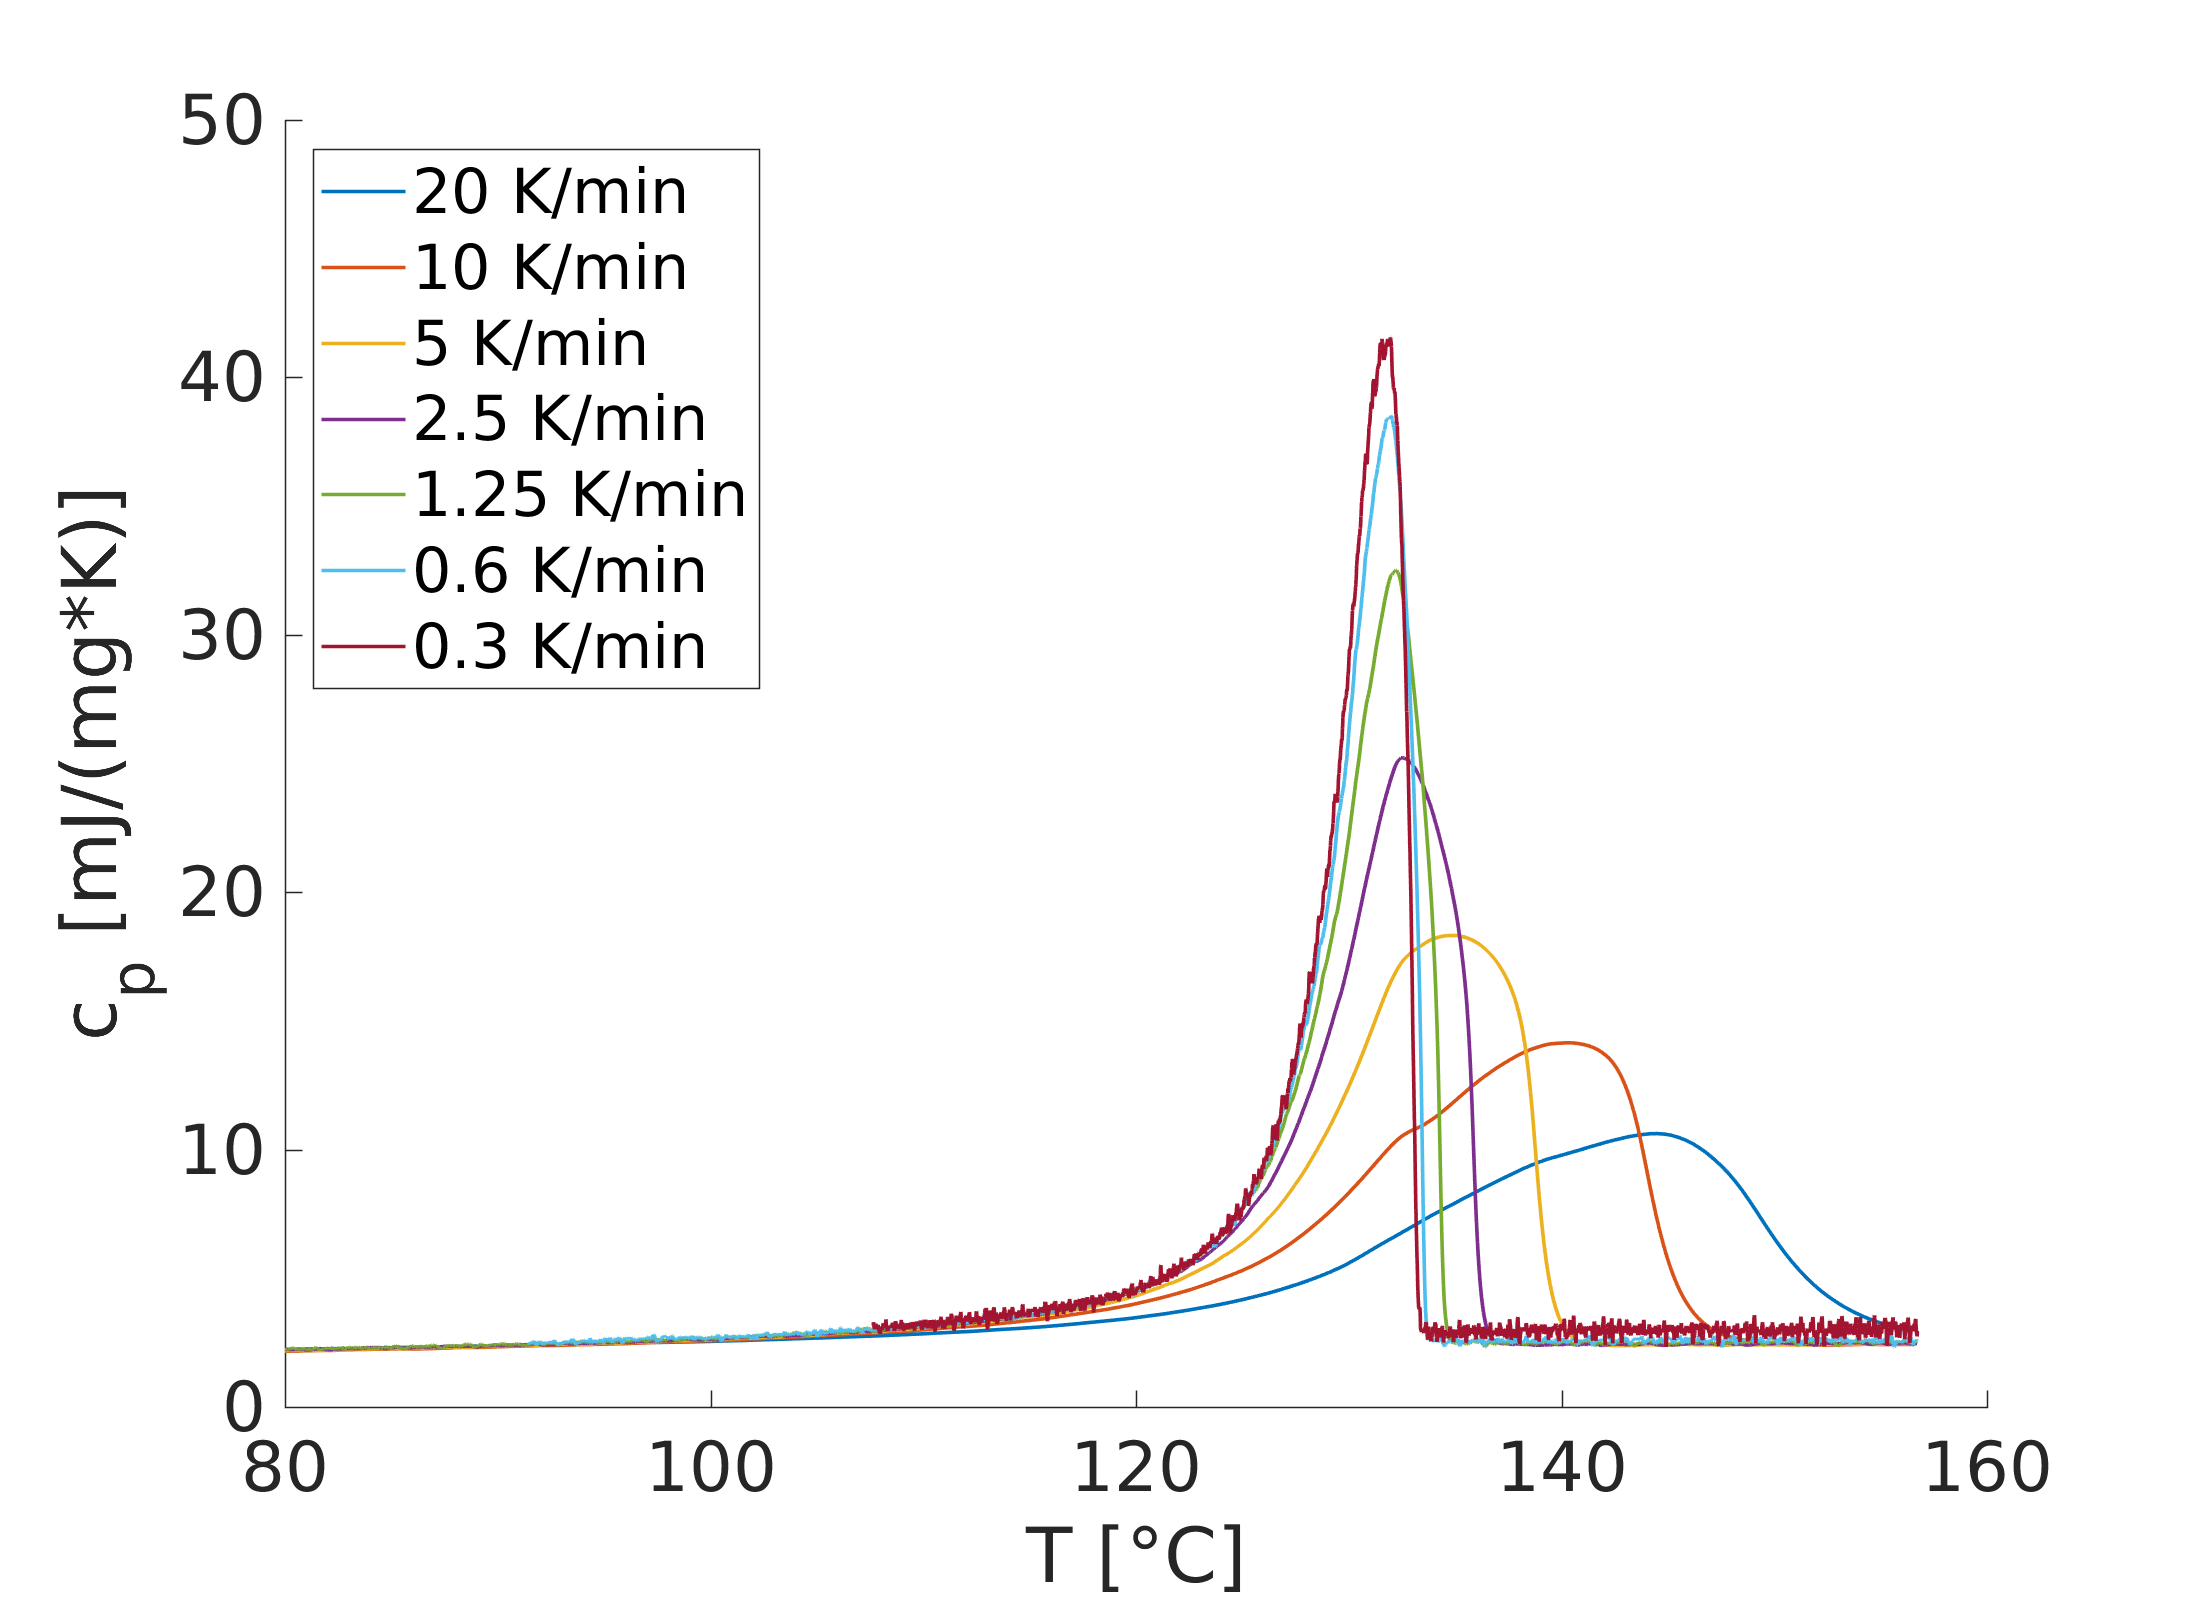
\includegraphics[width=0.7\textwidth]{/home/argo/masterarbeit/vortrag/images/c_p_DIN_formula.png}
	\end{textblock}
	
	\begin{textblock}{14}(1,12.5)
		\begin{equation}
			\text{DIN 11357: } \quad c_p^S(T) = c_p^{R}(T) \cdot \frac{m^R}{m^S} \cdot \frac{\Phi^S(T) - \Phi^0(T)}{\Phi^R(T) - \Phi^0(T)}
		\end{equation}
	\end{textblock}
	
}


\section{Parameter Estimation}
\subsection{Mathematical model}
\frame{
	\frametitle{Mathematical model}
	
	\begin{textblock}{14}(1, 4.6)
		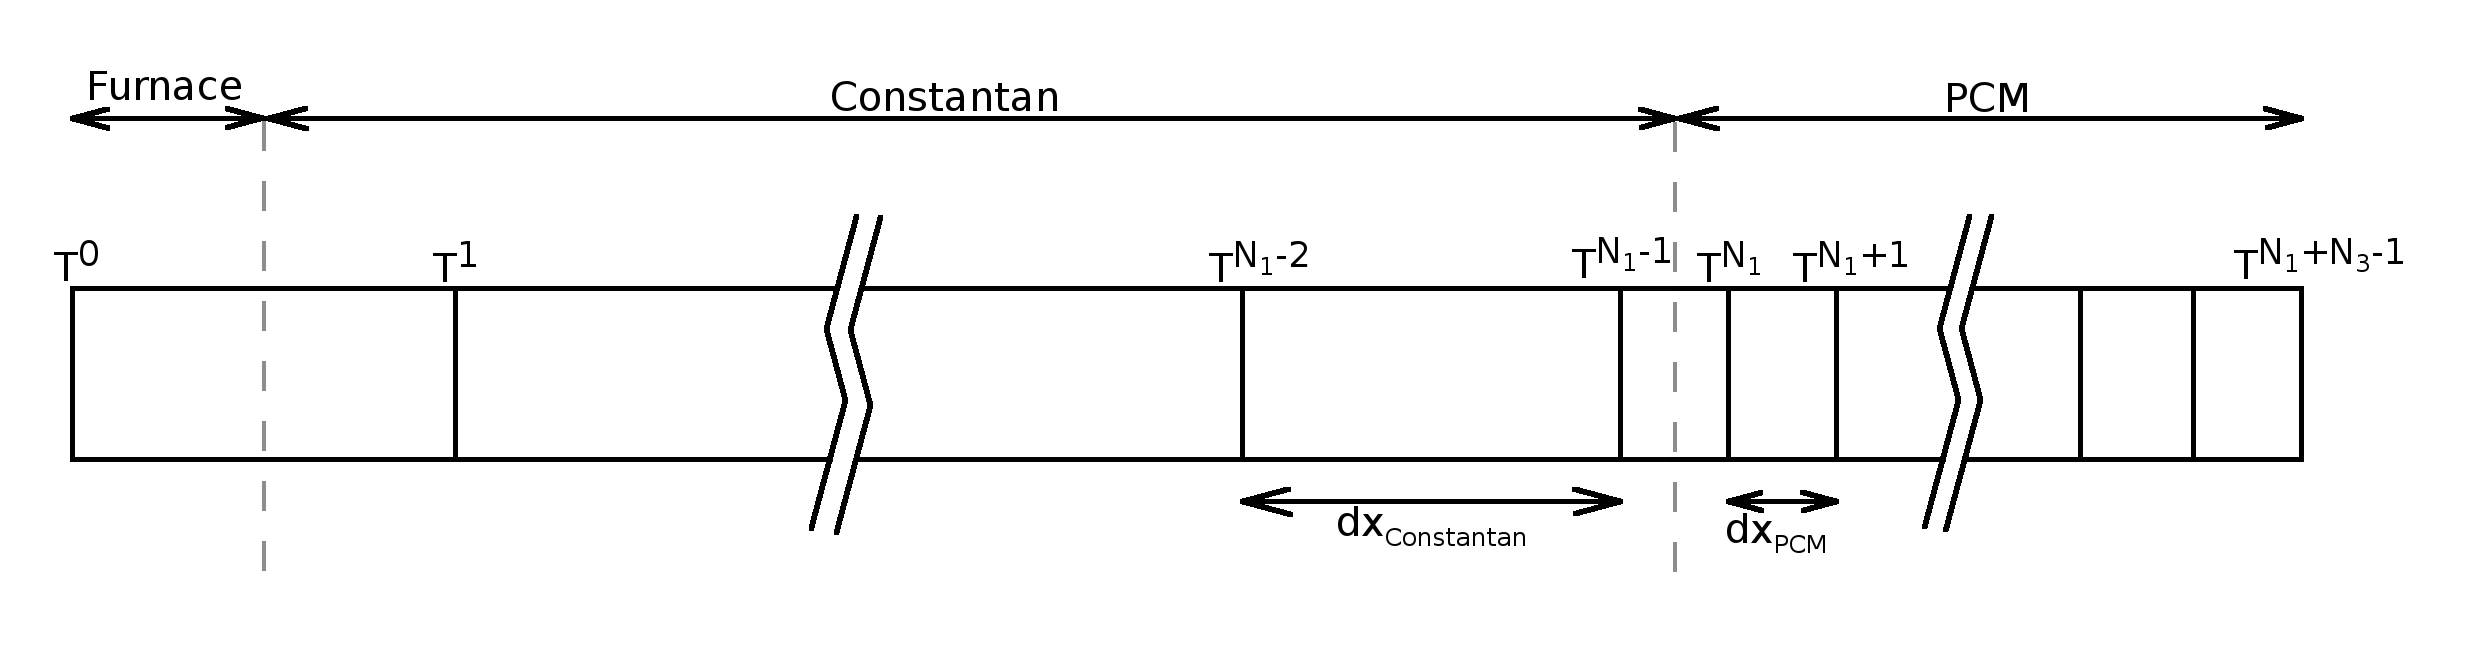
\includegraphics[width=1.\textwidth]{/home/argo/masterarbeit/thesis/images/discretization_grid.png}
	\end{textblock}
	
	
	\begin{textblock}{14}(1, 9.5)
	
		\begin{itemize}
			\item Heat equation: \quad $\rho c_p(T(x,t)) \frac{\partial T}{\partial t}(x,t) = \nabla \cdot \left[ \lambda \cdot \nabla T(x,t) \right]$
			\item $\rho$, $\lambda$ constant
			\item Boundary conditions: 
				\begin{itemize}
				\item $T^0 = T_{\text{start}} + \beta \cdot t$ \\
				\item No flux outside PCM
				\end{itemize}
			\item Reference and PCM side are independent
			
		\end{itemize}
	\end{textblock}

	
}


\frame{
	\frametitle{Mathematical Model}

	\begin{textblock}{14}(1.5, 3.8)
	
		\begin{align*}
		\hspace{-1cm}
		\frac{d}{dt} \begin{bmatrix*}
		T^0 \\[1ex]
		T^1 \\[0.3ex]
		\vdots \\[1ex]
		T^{N_1-2} \\[1.7ex]
		T^{N_1-1} \\[1.7ex]
		T^{N_1} \\[0.5ex]
		\vdots \\[1.5ex]
		T^{N_1+N_3-2} \\[1ex]
		T^{N_1+N_3-1}
		\end{bmatrix*} =
		\begin{bmatrix}
		\beta \\
		\frac{\lambda^{\text{Ag}}}{\rho^{\text{Ag}} \ c_p^{\text{Ag}}} \cdot \frac{T^{0} - 2 T^{1} + T^{2}}{\Delta x_{\text{Ag}}^2} \\
		\vdots \\
		\frac{\lambda^{\text{Ag}}}{\rho^{\text{Ag}} \ c_p^{\text{Ag}}} \cdot \frac{T^{N_1-3} - 2 T^{N_1-2} + T^{N_1-1}}{\Delta x_{\text{Ag}}^2} \\
		\frac{\lambda^{\text{Ag}}}{\rho^{\text{Ag}} \ c_p^{\text{Ag}}} \cdot \frac{\frac{2}{1+\alpha} T^{N_1-2} - \frac{2}{\alpha} T^{N_1-1} + \frac{2}{\alpha (\alpha + 1)} T^{N_1}}{\Delta x_{\text{Ag}}^2} \\
		\frac{\lambda^{\text{PCM}}}{\rho^{\text{PCM}} \ c_p^{\text{PCM}}(T^{N^1})} \cdot \frac{T^{N_1-1} - 2 T^{N_1} + T^{N_1+1}}{\Delta x_{\text{PCM}}^2} \\
		\vdots \\
		\frac{\lambda^{\text{PCM}}}{\rho^{\text{PCM}} \ c_p^{\text{PCM}}(T^{N^1+N^3-2})} \cdot \frac{T^{N_1+N_3-3} - 2 T^{N_1+N_3-2} + T^{N_1+N_3-1}}{\Delta x_{\text{PCM}}^2} \\
		\frac{\lambda^{\text{PCM}}}{\rho^{\text{PCM}} \ c_p^{\text{PCM}}(T^{N^1+N^3-1})} \cdot \frac{T^{N_1+N_3-2} - T^{N_1+N_3-1}}{\Delta x_{\text{PCM}}^2}
		\end{bmatrix}
	\end{align*}

	\end{textblock}
}






\subsection{Parametrization $c_p$}
\frame{
	\frametitle{Parametrization $c_p$}
	
	\begin{textblock}{14}(1,5)
		
		\begin{equation*}
			c_p(T) = \sum_{i=1}^{10} A_i \exp\left(- \frac{(T - T_{\text{offset}_i})^2}{\sigma_i^2}\right) + m \cdot T + b
		\end{equation*}
		
		\centering
		\includegraphics[width=0.5\textwidth]{/home/argo/masterarbeit/fits_data/old_Constantan/2017-10-05_00:14:13_407_0,3Kmin_L1=15_L3=0,35/c_p(T).png}
		
	\end{textblock}
	
}



\frame{
	\frametitle{Numerical Solution of heat equation}
	
	\begin{textblock}{14}(1,5)
		\begin{itemize}
			\item Spatial discretization by method of lines
			\item Software: SolvIND using integrator DAESOL-II \\ \vspace{0.15cm}
			$\rightarrow$ Gives as well needed sensitivities $\frac{\partial T}{\partial p}$ for optimization \\
			\qquad via IND forward mode
			\item Used Relative Tolerance: $10^{-7}$
		\end{itemize}
	\end{textblock}	
}


\subsection{Optimization problem}
\frame{
	\frametitle{Heat flux computation}	
	
	\begin{textblock}{14}(1,5)
		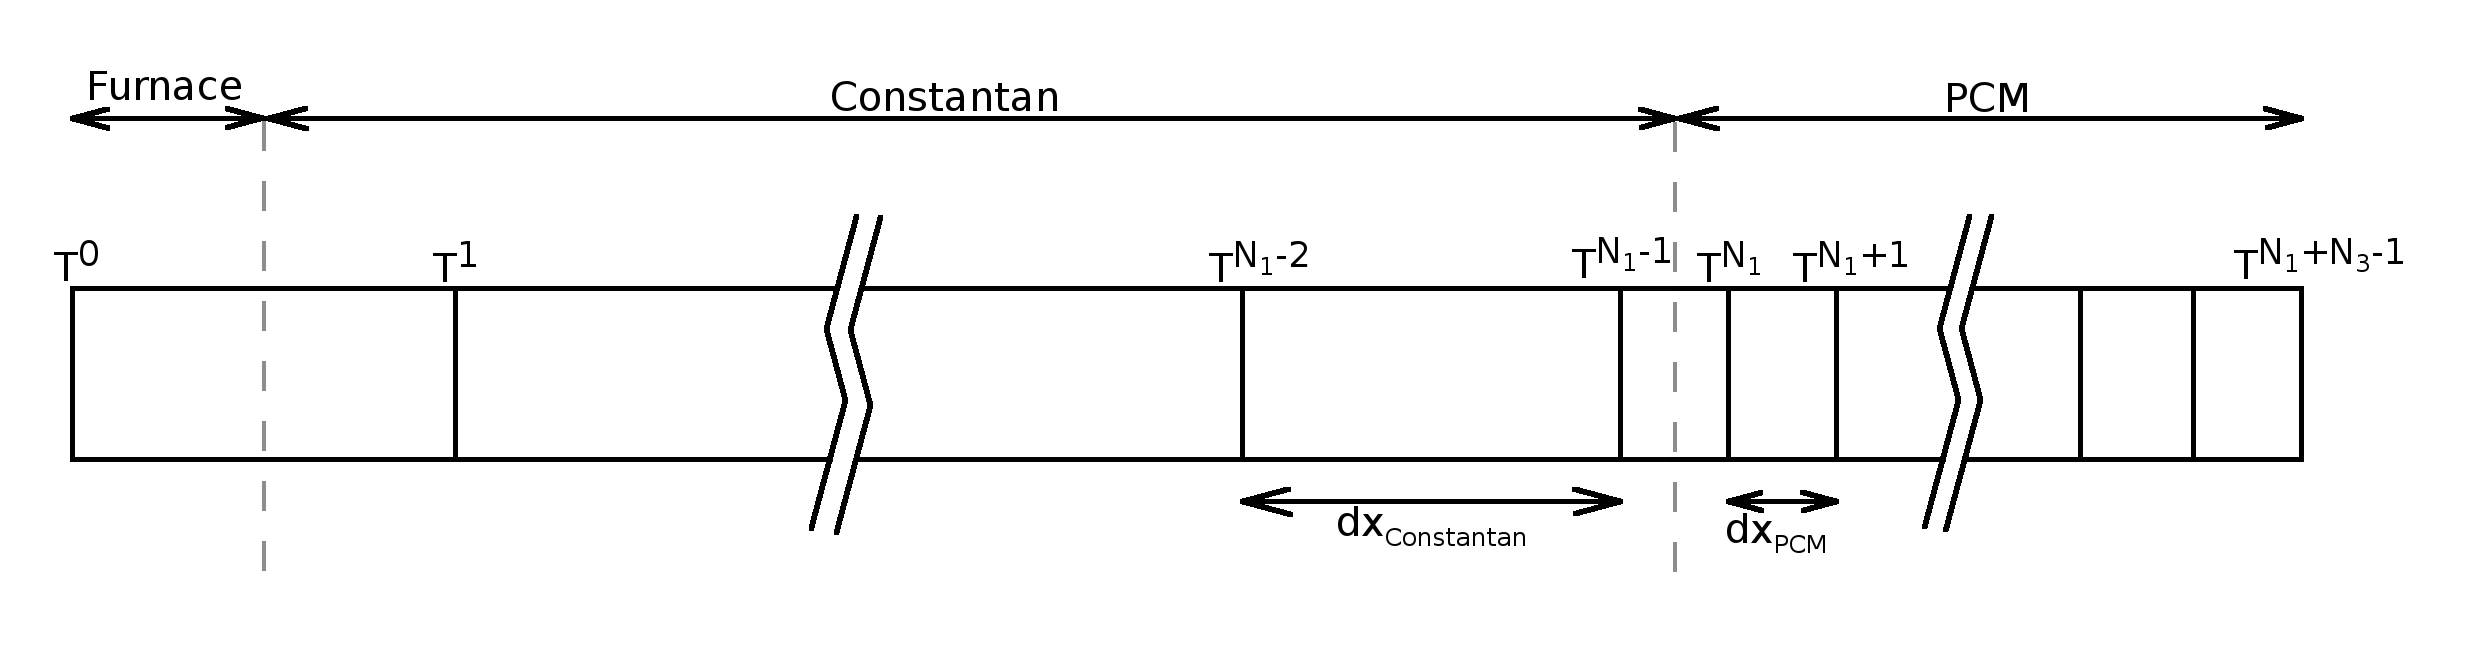
\includegraphics[width=1.\textwidth]{/home/argo/masterarbeit/thesis/images/discretization_grid.png}
	\end{textblock}
	
	\begin{textblock}{14}(1, 10)
		\begin{itemize}
			\item Heat flux into PCM: \\ \vspace{0.15cm}
			$\Phi_{q}^{PCM,in} = - \bar{\lambda} \frac{T^{N_1} - T^{N_1-1}}{dx_{PCM}} \cdot A_{PCM}
			\approx - \lambda_{PCM} \frac{T^{N_1+1} - T^{N_1}}{dx_{PCM}} \cdot A_{PCM}$ \\ \vspace{0.15cm}
			where for the cross section $A_{PCM}$ we used $m_i = \rho \cdot A \cdot dx_i$
		\end{itemize}
	\end{textblock}
	
}


\frame{
	\frametitle{Measurement times computation}
	
	
	
}



\frame{
	\frametitle{Optimization problem}	


	\begin{textblock}{10}(0.5,4.)
	\begin{align*}
		\min_{p_{c_p}} \ & \sum_{i=1}^{n_{MP}} \left|\left|  \Phi_{q}^{PCM,in}(T(t_i;T_0,p_{c_p})) - \eta_i^{\Phi} \right|\right|_2^2 \\
		s.t. \ & \quad \  \dot{T} = f(T,t;p_{c_p}) \\
		       & T(0) = T_0
	\end{align*}
	\end{textblock}
	
	\begin{textblock}{7}(11,7)
		$\forall$ heat rates $\beta$
	\end{textblock}
	
	\begin{textblock}{16}(0.3,9.4)
	\begin{itemize}
		\item $\eta_i^{\Phi}$: heat flux measurement value at time $t_i$
		\item $\Phi_q^{\text{PCM,in}}$: heat flux into PCM from simulation \\
		\item $n_{MP}$: number of measurement points \\
		\item $p_{c_p}$: optimization parameters specifying specific heat capacity $c_p(T)$ \\
		\item $f(T,t;p_{c_p})$: discretized differential equation system from heat equation
	\end{itemize}
	
	\end{textblock}

	
}





\subsection{Results}
\frame{
	\frametitle{Results}
	\begin{textblock}{14}(1,5)
		\centering
		Heat rate: $20\frac{K}{min}$
	\end{textblock}
	
	\begin{textblock}{14}(1,6)
		\includegraphics[width=0.5\textwidth]{/home/argo/masterarbeit/fits_data/2017-10-18_16:40:21_407_L1=40_L3=0.1_N1=500_N3=50/2017-10-18_16:44:17_407_20Kmin_L1=40_L3=0,1/c_p(T).png}
	\end{textblock}
	
	\begin{textblock}{14}(8,6)
		\includegraphics[width=0.5\textwidth]{/home/argo/masterarbeit/fits_data/2017-10-18_16:40:21_407_L1=40_L3=0.1_N1=500_N3=50/2017-10-18_16:44:17_407_20Kmin_L1=40_L3=0,1/q_pcm_in(T_ref).png}
	\end{textblock}	
}


\frame{
	\frametitle{Results}
	\begin{textblock}{14}(1,5)
		\centering
		Heat rate: $10\frac{K}{min}$
	\end{textblock}
	
	\begin{textblock}{14}(1,6)
		\includegraphics[width=0.5\textwidth]{/home/argo/masterarbeit/fits_data/2017-10-18_16:40:21_407_L1=40_L3=0.1_N1=500_N3=50/2017-10-18_16:55:30_407_10Kmin_L1=40_L3=0,1/c_p(T).png}
	\end{textblock}
	
	\begin{textblock}{14}(8,6)
		\includegraphics[width=0.5\textwidth]{/home/argo/masterarbeit/fits_data/2017-10-18_16:40:21_407_L1=40_L3=0.1_N1=500_N3=50/2017-10-18_16:55:30_407_10Kmin_L1=40_L3=0,1/q_pcm_in(T_ref).png}
	\end{textblock}	
}


\frame{
	\frametitle{Results}
	\begin{textblock}{14}(1,5)
		\centering
		Heat rate: $5\frac{K}{min}$
	\end{textblock}
	
	\begin{textblock}{14}(1,6)
		\includegraphics[width=0.5\textwidth]{/home/argo/masterarbeit/fits_data/2017-10-18_16:40:21_407_L1=40_L3=0.1_N1=500_N3=50/2017-10-18_17:12:14_407_5Kmin_L1=40_L3=0,1/c_p(T).png}
	\end{textblock}
	
	\begin{textblock}{14}(8,6)
		\includegraphics[width=0.5\textwidth]{/home/argo/masterarbeit/fits_data/2017-10-18_16:40:21_407_L1=40_L3=0.1_N1=500_N3=50/2017-10-18_17:12:14_407_5Kmin_L1=40_L3=0,1/q_pcm_in(T_ref).png}
	\end{textblock}	
}



\frame{
	\frametitle{Results}
	\begin{textblock}{14}(1,5)
		\centering
		Heat rate: $0.3\frac{K}{min}$
	\end{textblock}
	
	\begin{textblock}{14}(1,6)
		\includegraphics[width=0.5\textwidth]{/home/argo/masterarbeit/fits_data/2017-10-18_16:40:21_407_L1=40_L3=0.1_N1=500_N3=50/2017-10-18_17:55:49_407_0,3Kmin_L1=40_L3=0,1/c_p(T).png}
	\end{textblock}
	
	\begin{textblock}{14}(8,6)
		\includegraphics[width=0.5\textwidth]{/home/argo/masterarbeit/fits_data/2017-10-18_16:40:21_407_L1=40_L3=0.1_N1=500_N3=50/2017-10-18_17:55:49_407_0,3Kmin_L1=40_L3=0,1/q_pcm_in(T_ref).png}
	\end{textblock}	
}






\frame{
	\frametitle{Results}
	\begin{textblock}{14}(1,5)
		\centering
		$c_p$ curves for all heat rates
	\end{textblock}
	
	\begin{textblock}{14}(1,6)
		\includegraphics[width=0.5\textwidth]{/home/argo/masterarbeit/fits_data/2017-10-18_16:40:21_407_L1=40_L3=0.1_N1=500_N3=50/c_p_all.png}
	\end{textblock}
	
	\begin{textblock}{14}(8,6)
		\includegraphics[width=0.5\textwidth]{/home/argo/masterarbeit/fits_data/2017-10-18_16:40:21_407_L1=40_L3=0.1_N1=500_N3=50/c_p_all_zoom.png}
	\end{textblock}	
}



\frame{
	\frametitle{Results}
	\begin{textblock}{14}(1,5)
		\centering
		Modifying silver / PCM length $L_1$ / $L_3$
	\end{textblock}
	
	\begin{textblock}{14}(1,6)
		\includegraphics[width=0.5\textwidth]{/home/argo/masterarbeit/fits_data/2017-10-18_10:59:34_407_L1=80_L3=0.1_N1=200_N3=50/c_p_all_zoom.png} \\
		
		\qquad \qquad  $L_1 = 80$, $L_3 = 0.1$
	\end{textblock}
	
	\begin{textblock}{14}(8,6)
		\includegraphics[width=0.5\textwidth]{/home/argo/masterarbeit/fits_data/2017-10-18_14:41:19_407_L1=40_L3=0.2_N1=200_N3=50/c_p_all_zoom.png} \\
		
		\qquad \qquad  $L_1 = 40$, $L_3 = 0.2$
	\end{textblock}	
}



\frame{
	\frametitle{Results}
	\begin{textblock}{14}(1,5)
		\centering
		Modifying silver / PCM length $L_1$ / $L_3$
	\end{textblock}
	
	\begin{textblock}{14}(1,6)
		\includegraphics[width=0.5\textwidth]{/home/argo/masterarbeit/fits_data/2017-10-15_21:08:00_407_L1=5_L3=0.1_N1=200_N3=50/c_p_all_zoom.png} \\
		
		\qquad \qquad  $L_1 = 5$, $L_3 = 0.1$
	\end{textblock}
	
	\begin{textblock}{14}(8,6)
		\includegraphics[width=0.5\textwidth]{/home/argo/masterarbeit/fits_data/2017-10-18_12:11:40_407_L1=40_L3=0.01_N1=200_N3=50/c_p_all_zoom.png} \\
		
		\qquad \qquad  $L_1 = 40$, $L_3 = 0.01$
	\end{textblock}	
}





\section{Next potential steps}
\frame{
	\frametitle{Next potential steps}
	
	\begin{itemize}
		\item Discretization transition from silver to PCM softer
		\item Heat equation with $\rho=\rho(T)$ \\
		$\rightarrow$ problem with value of absolute enthalpy term
		\item $L_1$ and $L_3$ as optimization variable \\
		$\rightarrow$ high programming effort
		\item Crucible part between silver and PCM \\
		$\rightarrow$ we do not know $L_2$ (risk of overfitting) \\
	\end{itemize}
	
}



\section{Open Questions}
\frame{
	\frametitle{Open Questions}
	
	\begin{itemize}
		\item Reason for shift in $c_p$ fits?
		\item Heat equation derivation with $\rho=\rho(T)$ correct? \\
		$\rightarrow$ How to get enthalpy $h$?
		\item How to get $L_1$ and $L_3$ except as optimization variable?
	\end{itemize}
	
}





	
	
\end{document}